\documentclass[12pt,border=0pt]{standalone}

\usepackage[utf8]{inputenc} 
\usepackage{amssymb,amsmath}
\usepackage{tikz}
\usetikzlibrary{positioning}
\usepackage{color}


\thispagestyle{empty}

\begin{document}

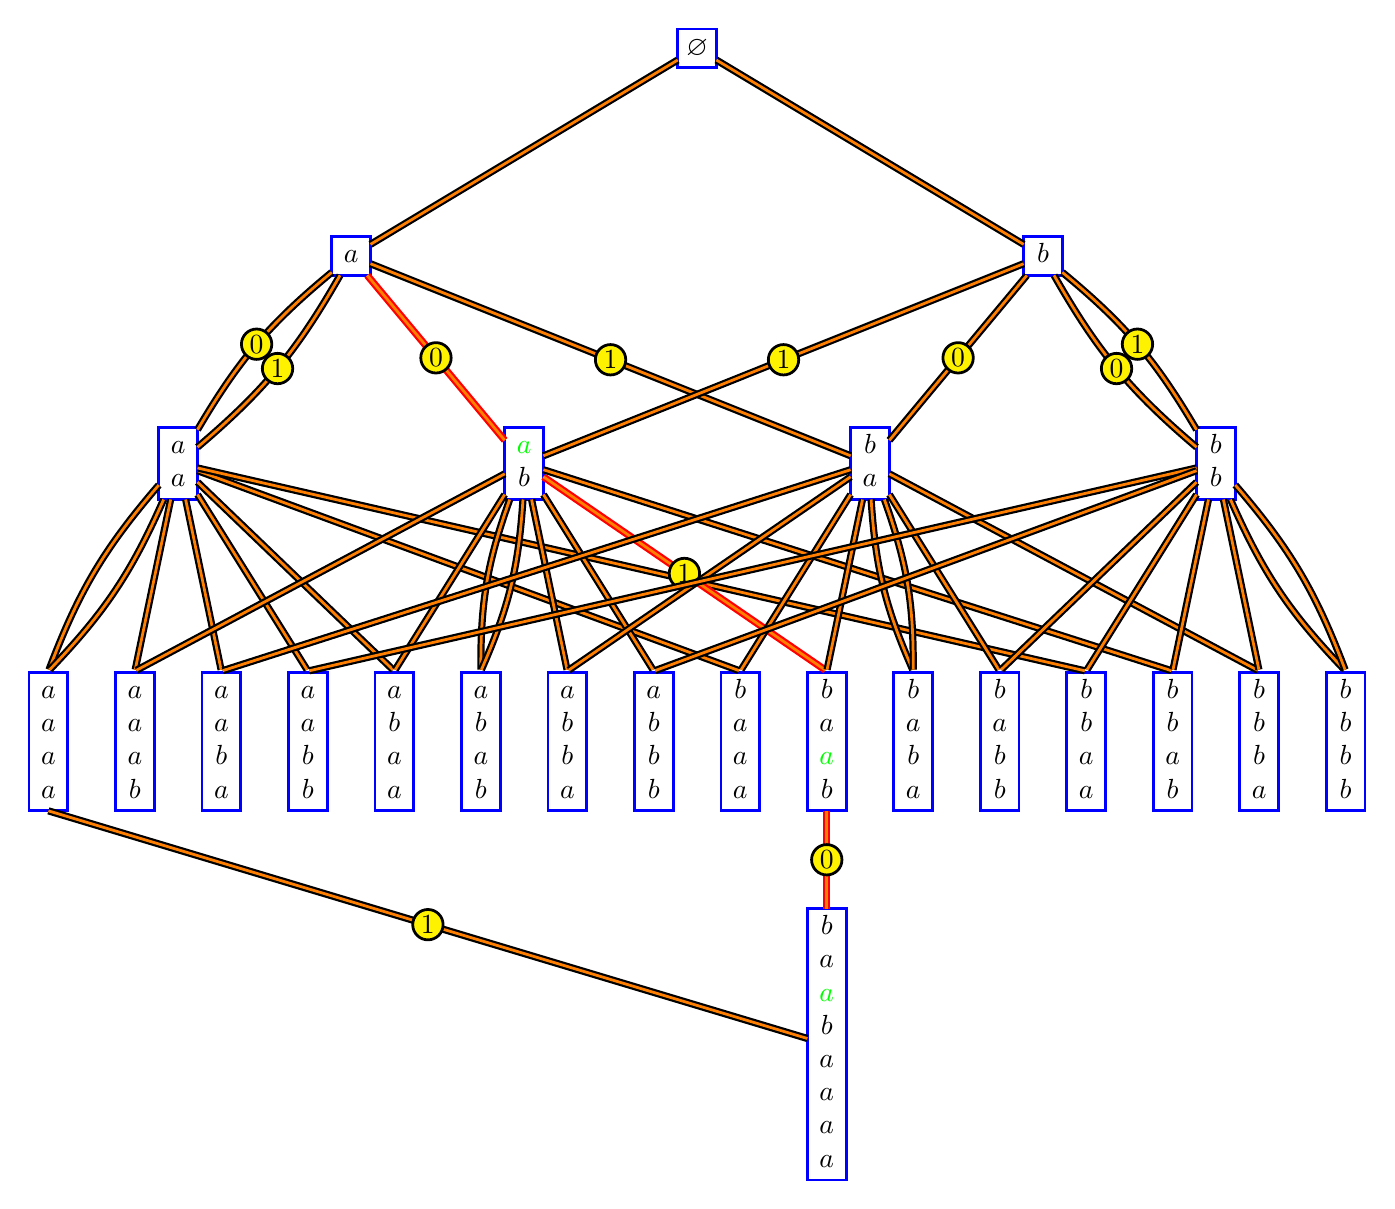
\begin{tikzpicture}[x=10pt,y=6pt]
  \centering
  \tikzset{VertexStyle/.style = {
    shape         = rectangle,
    draw          = blue, 
    fill          = white, 
  	line width    = 1pt, 
    text          = black,
    inner sep     = 1pt,
    outer sep     = 0pt,
    minimum size  = 14 pt,
    scale         = 1
    }
  }
  \tikzset{EmptyStyle/.style = {
    shape         = rectangle,
    draw          = white, 
    fill          = white, 
  	line width    = 0pt, 
    inner sep     = 0pt,
    outer sep     = 0pt,
    scale         = 1
    }
  }
  \tikzset{EdgeStyle/.style = {
    draw            = black, 
    thick,
    double          = orange,
    double distance = 1pt
    }
  }
  \tikzset{EdgeLabelStyle/.style = {
    draw          = black,
  	shape         = circle, 
  	line width    = 1pt, 
  	minimum size  = 10pt, 
    inner sep     = 1pt,
    outer sep     = 0pt,
    fill          = yellow,
    text          = black,
    scale         = 1
    }
  }

	\node[VertexStyle](A1) at (25, 43.75) {$\varnothing$};
	\node[VertexStyle](B1) at (12.5, 31.25) {$\begin{matrix} a \end{matrix}$};
	\node[VertexStyle](B2) at (37.5, 31.25) {$\begin{matrix} b \end{matrix}$};
	\node[VertexStyle](C1) at (6.25, 18.75) {$\begin{matrix} a\\ a \end{matrix}$};
	\node[VertexStyle](C2) at (18.75, 18.75) {$\begin{matrix} {\color{green}a}\\ b \end{matrix}$};
	\node[VertexStyle](C3) at (31.25, 18.75) {$\begin{matrix} b\\ a \end{matrix}$};
	\node[VertexStyle](C4) at (43.75, 18.75) {$\begin{matrix} b\\ b \end{matrix}$};
	%
	\node[EmptyStyle](D01) at (1.5625, 6.25) {};
	\node[EmptyStyle](D02) at (4.6875, 6.25) {};
	\node[EmptyStyle](D03) at (7.8125, 6.25) {};
	\node[EmptyStyle](D04) at (10.9375, 6.25) {};
	\node[EmptyStyle](D05) at (14.0625, 6.25) {};
	\node[EmptyStyle](D06) at (17.1875, 6.25) {};
	\node[EmptyStyle](D07) at (20.3125, 6.25) {};
	\node[EmptyStyle](D08) at (23.4375, 6.25) {};
	\node[EmptyStyle](D09) at (26.5625, 6.25) {};
	\node[EmptyStyle](D10) at (29.6875, 6.25) {};
	\node[EmptyStyle](D11) at (32.8125, 6.25) {};
	\node[EmptyStyle](D12) at (35.9375, 6.25) {};
	\node[EmptyStyle](D13) at (39.0625, 6.25) {};
	\node[EmptyStyle](D14) at (42.1875, 6.25) {};
	\node[EmptyStyle](D15) at (45.3125, 6.25) {};
	\node[EmptyStyle](D16) at (48.4375, 6.25) {};
	%
	\node[VertexStyle, below=0 of D01](bD01) {$\begin{matrix} a\\ a\\ a\\ a \end{matrix}$};
	\node[VertexStyle, below=0 of D02](bD02) {$\begin{matrix} a\\ a\\ a\\ b \end{matrix}$};
	\node[VertexStyle, below=0 of D03](bD03) {$\begin{matrix} a\\ a\\ b\\ a \end{matrix}$};
	\node[VertexStyle, below=0 of D04](bD04)  {$\begin{matrix} a\\ a\\ b\\ b \end{matrix}$};
	\node[VertexStyle, below=0 of D05](bD05)  {$\begin{matrix} a\\ b\\ a\\ a \end{matrix}$};
	\node[VertexStyle, below=0 of D06](bD06)  {$\begin{matrix} a\\ b\\ a\\ b \end{matrix}$};
	\node[VertexStyle, below=0 of D07](bD07)  {$\begin{matrix} a\\ b\\ b\\ a \end{matrix}$};
	\node[VertexStyle, below=0 of D08](bD08)  {$\begin{matrix} a\\ b\\ b\\ b \end{matrix}$};
	\node[VertexStyle, below=0 of D09](bD09)  {$\begin{matrix} b\\ a\\ a\\ a \end{matrix}$};
	\node[VertexStyle, below=0 of D10](bD10)  {$\begin{matrix} b\\ a\\ {\color{green}a}\\ b \end{matrix}$};
	\node[VertexStyle, below=0 of D11](bD11) {$\begin{matrix} b\\ a\\ b\\ a \end{matrix}$};
	\node[VertexStyle, below=0 of D12](bD12)  {$\begin{matrix} b\\ a\\ b\\ b \end{matrix}$};
	\node[VertexStyle, below=0 of D13](bD13)  {$\begin{matrix} b\\ b\\ a\\ a \end{matrix}$};
	\node[VertexStyle, below=0 of D14](bD14)  {$\begin{matrix} b\\ b\\ a\\ b \end{matrix}$};
	\node[VertexStyle, below=0 of D15](bD15)  {$\begin{matrix} b\\ b\\ b\\ a \end{matrix}$};
	\node[VertexStyle, below=0 of D16](bD16)  {$\begin{matrix} b\\ b\\ b\\ b \end{matrix}$};

	\node[VertexStyle, below=3cm of D10](EE)  {$\begin{matrix} b\\ a\\ {\color{green}a}\\ b \\ a \\ a \\ a \\ a \end{matrix}$};
	\draw[EdgeStyle, red](bD10) to node[EdgeLabelStyle]{$0$} (EE);
	\draw[EdgeStyle](bD01.south) to node[EdgeLabelStyle]{$1$} (EE);

	%
	\draw[EdgeStyle](A1) to (B1);
	\draw[EdgeStyle](A1) to (B2);
	\draw[EdgeStyle, bend left=-10](B1) to node[EdgeLabelStyle]{$0$} (C1);
	\draw[EdgeStyle, bend left=10](B1) to node[EdgeLabelStyle]{$1$} (C1);
	\draw[EdgeStyle, red](B1) to node[EdgeLabelStyle]{$0$} (C2);
	\draw[EdgeStyle](B1) to node[EdgeLabelStyle]{$1$} (C3);
	\draw[EdgeStyle](B2) to node[EdgeLabelStyle]{$1$} (C2);
	\draw[EdgeStyle](B2) to node[EdgeLabelStyle]{$0$} (C3);
	\draw[EdgeStyle, bend left=-10](B2) to node[EdgeLabelStyle]{$0$} (C4);
	\draw[EdgeStyle, bend left=10](B2) to node[EdgeLabelStyle]{$1$} (C4);
	\draw[EdgeStyle, bend left=-10](C1) to (D01);
	\draw[EdgeStyle, bend left=10](C1) to (D01);
	\draw[EdgeStyle](C1) to (D02);
	\draw[EdgeStyle](C1) to (D03);
	\draw[EdgeStyle](C1) to (D04);
	\draw[EdgeStyle](C1) to (D05);
	\draw[EdgeStyle](C1) to (D09);
	\draw[EdgeStyle](C1) to (D13);
	\draw[EdgeStyle](C2) to (D02);
	\draw[EdgeStyle](C2) to (D05);
	\draw[EdgeStyle, bend left=-10](C2) to (D06);
	\draw[EdgeStyle, bend left=10](C2) to (D06);
	\draw[EdgeStyle](C2) to (D07);
	\draw[EdgeStyle](C2) to (D08);
	\draw[EdgeStyle, red](C2) to node[EdgeLabelStyle]{$1$} (D10);
	\draw[EdgeStyle](C2) to (D14);
	\draw[EdgeStyle](C3) to (D03);
	\draw[EdgeStyle](C3) to (D07);
	\draw[EdgeStyle](C3) to (D09);
	\draw[EdgeStyle](C3) to (D10);
	\draw[EdgeStyle, bend left=-10](C3) to (D11);
	\draw[EdgeStyle, bend left=10](C3) to (D11);
	\draw[EdgeStyle](C3) to (D12);
	\draw[EdgeStyle](C3) to (D15);
	\draw[EdgeStyle](C4) to (D04);
	\draw[EdgeStyle](C4) to (D08);
	\draw[EdgeStyle](C4) to (D12);
	\draw[EdgeStyle](C4) to (D13);
	\draw[EdgeStyle](C4) to (D14);
	\draw[EdgeStyle](C4) to (D15);
	\draw[EdgeStyle, bend left=-10](C4) to (D16);
	\draw[EdgeStyle, bend left=10](C4) to (D16);
	
%	  \node[left=5cm of B1] (n0) {$n=0$};
%	  \node[below=2cm of n0] (n1) {$n=-1$};
%	  \node[below=3cm of n1] {$n=-2$};



  \end{tikzpicture}

\end{document}
